\documentclass[a4paper,titlepage]{article}
\usepackage{amssymb}
\usepackage[OT4,plmath]{polski}
\usepackage[polish]{babel}
\usepackage{csquotes}
\DeclareQuoteAlias{croatian}{polish} % cudzysłowy w bibliografii
\usepackage[style=numeric,sorting=nty,isbn=false,abbreviate = false,backend=biber]{biblatex}
\usepackage[margin=1in]{geometry}
\usepackage[noend]{algpseudocode}
\usepackage[page]{appendix}
\usepackage[usenames,dvipsnames,svgnames,table]{xcolor}
\usepackage[utf8]{inputenc}
\usepackage{adjustbox}
\usepackage{algorithm}
\usepackage{amsfonts}
\usepackage{amsmath}
\usepackage{amsthm}
\usepackage{array}
\usepackage{enumitem}
\usepackage{graphicx}
\usepackage{hyperref}
%\usepackage{indentfirst}
\usepackage{longtable}
\usepackage{multirow}
\usepackage{parskip}
\usepackage{pifont}
\usepackage{setspace}
\usepackage{verbatimbox}
\usepackage{wrapfig}
\usepackage{bm}
\usepackage{mathtools}

\linespread{1.4}

\renewcommand*\appendixpagename{Załącznik}
\renewcommand{\qedsymbol}{$\square$}
\renewcommand{\algorithmiccomment}[1]{\hfill\textcolor{black!65}{\textit{#1}}}
\let\emptyset\varnothing

\makeatother
%\setlength{\parindent}{24pt}
\theoremstyle{break}
\newtheorem*{uwaga}{Uwaga}
\newtheorem{definicja}{Definicja}[section]
\newtheorem{ozn}{Oznaczenie}[section]

\newcommand{\cmark}{\textcolor{ForestGreen}{\ding{51}}}
\newcommand{\xmark}{\textcolor{Maroon}{\ding{55}}}

\numberwithin{equation}{subsection}
\addbibresource{Dokumentacja.bib}

%------------------------------------------------------------------------------

\title{Dokumentacja projektu}
\author{
    \href{mailto:bezap@student.mini.pw.edu.pl}{Patryk~Bęza}\\[0.7em]
    \href{mailto:kozakm@student.mini.pw.edu.pl}{Marek~Kozak}\\[0.7em]
    \href{mailto:malasnickik@student.mini.pw.edu.pl}{Krzysztof~Małaśnicki}\\[0.7em]
}
\date{\today}

\begin{document}

\makeatletter
\renewcommand{\ALG@name}{Algorytm}
\begin{titlepage}
\newcommand{\HRule}{\rule{\linewidth}{0.5mm}}
\center


\includegraphics[width=2.0cm]{img/mini}\\[1.5cm]
\textsc{\LARGE Politechnika Warszawska}\\[0.3cm]
\textsc{\Large Wydział Matematyki i~Nauk Informacyjnych}\\[1.5cm]
\textsc{\large Komputerowe wspomaganie technik kryminalistycznych}\\[0.2cm]
\textsc{\small Rok akademicki 2015/2016}\\[1.5cm]

\HRule \\[1cm]
{ \huge \bfseries \@title}\\[0.7cm]
\HRule \\[1.75cm]

\begin{minipage}[t]{0.4\textwidth}
\begin{flushleft}\large
\textsc{Autorzy:}\\[3mm]
\@author
\end{flushleft}
\end{minipage}
\begin{minipage}[t]{0.4\textwidth}
\begin{flushright}\large
\textsc{Wykładowca:}\\[3mm]
\href{mailto:m.szezynska@ise.pw.edu.pl}{dr~inż.~Magdalena~Szeżyńska}\\[1cm]
\end{flushright}
\end{minipage}
\vfill
{\large \today}

\end{titlepage}

%\maketitle
\tableofcontents
\clearpage

%------------------------------------------------------------------------------

\begin{abstract}

\begin{figure}[t]
    \centering
    \hspace{-2em}
    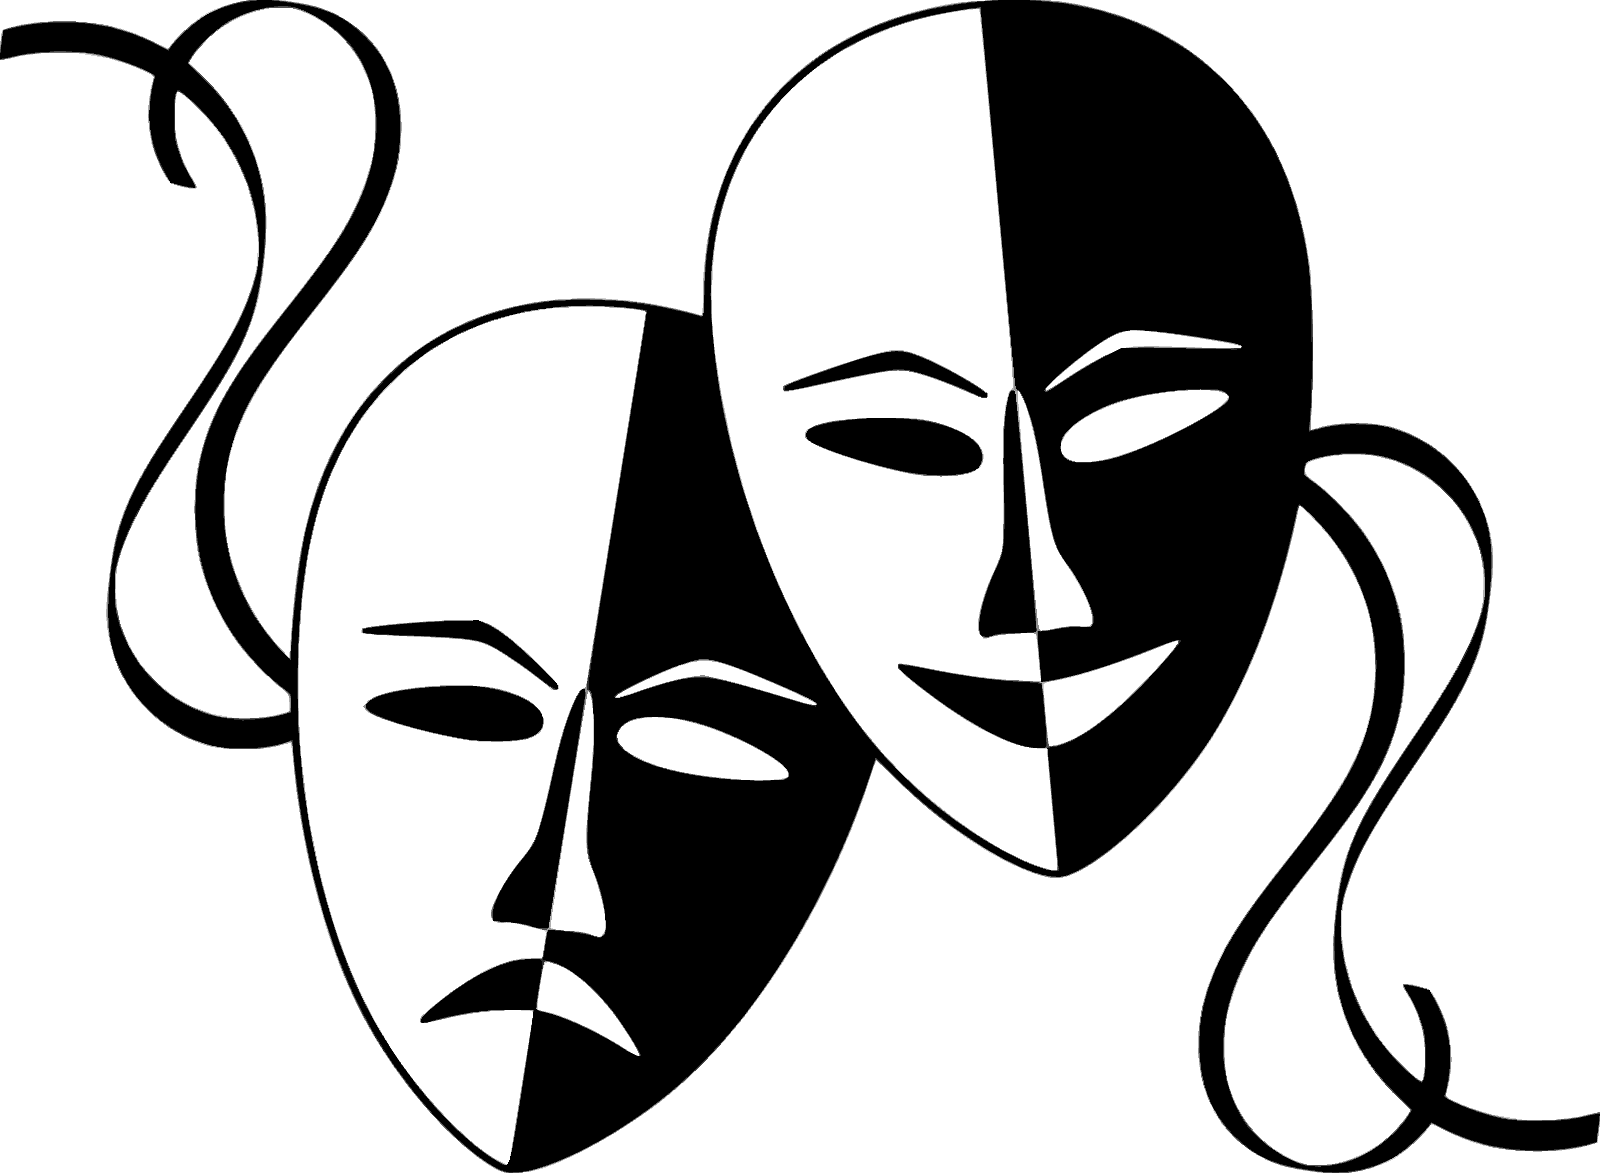
\includegraphics[width=0.45\textwidth]{img/faces}
\end{figure}

Niniejszy dokument powstał w~ramach dokumentacji projektu zespołowego z~przedmiotu \emph{\href{http://staff.elka.pw.edu.pl/~mszezyns/CAF/index.html}{Komputerowe wspomaganie technik kryminalistycznych}} w semestrze letnim roku akademickiego~2015/2016 na \emph{\href{http://www.mini.pw.edu.pl/}{Wydziale MiNI}~\href{https://www.pw.edu.pl/}{Politechniki Warszawskiej}}. Ma on za zadanie udokumentować ideę działania aplikacji identyfikującą twarze, uzasadnienie wyboru zastosowanych algorytmów, sposób jej użycia, wykorzystane narzędzia i biblioteki, wyniki testów funkcjonalnych i wydajnościowych oraz wnioski.

\end{abstract}

\clearpage

%------------------------------------------------------------------------------

\section{Wstęp}
\label{sec:wstep}

W tym rozdziale przedstawiono założenia wstępne projektu pt.~,,Identyfikacja twarzy".

%------------------------------------------------------------------------------

\subsection{Identyfikacja twarzy}

Identyfikacja twarzy to przypisanie tożsamości do dwu- lub trzywymiarowego zdjęcia twarzy. Przez ostatnie kilkadziesiąt lat opracowano wiele algorytmów, które służą do rozpoznawania i identyfikacji twarzy. Część z nich jest oparta na sieciach neuronowych, a pozostała część korzysta z klasycznych metod aparatu matematycznego, np. algebry i analizy statystycznej.

W ramach niniejszego projektu powstało rozwiązanie oparte o metody klasyczne, oparte na algebrze, a w szczególności na wyliczaniu wartości własnych i wektorów własnych macierzy, powstałej z analizowanych zdjęć twarzy, celem zamodelowania analizowanych zdjęć w przestrzeni liniowej, rozpiętej przez wyliczone wektory własne. Wykorzystana metoda identyfikacji twarzy to metoda~\emph{eigenfaces}, która opiera się na metodzie analizy głównych składowych~(ang.~\emph{Principal Component Analysis} -- w~skrócie:~PCA).

%------------------------------------------------------------------------------

\subsection{Zastosowania identyfikacji twarzy}

Istnieje wiele zastosowań identyfikacji twarzy. Część z nich dotyczy zastosowań w rozrywce, takiej jak np. gry czy identyfikacja twarzy na zdjęciach serwisów społecznościowych\footnote{W przeciwieństwie do rozpoznawania twarzy, identyfikacja twarzy nie jest jeszcze stosowana na szeroką skalę na największych serwisach społecznościowych.}. Poza zastosowaniami identyfikacji twarzy w rozrywce, istnieją zastosowania do poważniejszych celów, np. do wspomagania technik kryminalistycznych i szeroko pojętego bezpieczeństwa danych, np.: systemy kontroli dostępu, systemy bezpieczeństwa na lotniskach, policyjne bazy danych osób poszukiwanych (np. zaginionych, poszukiwanych listami gończymi i podejrzanych).

Identyfikacja twarzy w komputerowym wspomaganiu technik kryminalistycznych jest ważnym zagadnieniem dla wszystkich służb dbających o bezpieczeństwo, które posiadają bazy danych ze zdjęciami twarzy tysięcy osób, wśród których może znajdować się zdjęcie osoby identyfikowanej, np. podejrzanej, poszukiwanej lub zaginionej. Niniejsza dokumentacja jest opisem szczegółów implementacyjnych aplikacji służącej do identyfikacji dwuwymiarowych zdjęć twarzy.

%------------------------------------------------------------------------------

\subsection{Cel aplikacji}

Celem aplikacji jest zidentyfikowanie zadanej twarzy na podstawie zbioru zdjęć osób z lokalnej bazy danych. Zakładamy, że zdjęcia są znormalizowane, tzn. wszystkie zdjęcia są monochromatyczne, mają jednakowe rozmiary, twarze sfotografowana są frontalnie, tzn.~\emph{en~face} i są wycentrowane.

Jeśli osoba, której twarz podano na wejście programu nie znajduje się w bazie danych, program powinien zwrócić kilka zdjęć najbardziej podobnych do zadanego wraz z oszacowaniem ich podobieństwa w skali od $0\%$ do $100\%$. W obu przypadkach zdjęcia znalezionych twarzy powinny być posortowane nierosnąco względem podobieństwa do zadanej twarzy.

W przeciwnym razie, tzn. jeśli zdjęcia osoby, której twarz została poddana identyfikacji, znajdują się w bazie, program powinien znaleźć tę twarz i przypisać wartość jej podobieństwa bliską $100\%$ (wartość oczekiwana $=100\%$) oraz ewentualnie kilka innych, podobnych twarzy, z odpowiednio mniejszym podobieństwem wyrażonym w skali od $0\%$ do $100\%$.

Pierwszorzędnym celem aplikacji \emph{nie} jest szybkie działanie, co można uzasadnić tym, że algorytmy mające na celu zidentyfikowanie osoby, powinny przede wszystkim nie dopuścić do przeoczenia osoby, która znajduje się w bazie danych. Tak postawione wymaganie na ogół wymusza zastosowania algorytmów, które działają względnie długo.

%------------------------------------------------------------------------------

\section{Algorytm}
\label{sec:algorytm}

Do rozpoznawania twarzy została zastosowana \emph{metoda analizy głównych składowych}~(ang.~\emph{Principal Component Analysis} -- w~skrócie:~PCA), zaproponowana niezależnie przez angielskiego matematyka \emph{Karla Pearson'a}~(1901) oraz ekonoma i statystyka \emph{Harolda Hotelling'a}~(1933).

W niniejszym dziale przedstawiono opis metody PCA oraz \emph{eigenfaces}, na podstawie publikacji autorów metody \emph{eigenfaces} -- prof.~\emph{Matthew Turk'a} i prof.~\emph{Alex'a Pentland'a}\cite{turk}.

%------------------------------------------------------------------------------

\subsection{Analiza głównych składowych}

Jednym z głównych problemów z jakim mamy do czynienia w identyfikacji twarzy ze zdjęć, jest ich duży wymiar. Dwuwymiarowe, monochromatyczne zdjęcie zdjęcie o wymiarach $p\times q$, rozpina przestrzeń $m=p\cdot q$-wymiarową. Zdjęcie o wymiarach $100\times 100$~pikseli, rozpina przestrzeń $10000$-wymiarową. Istnieje potrzeba zmniejszenia tej przestrzeni kosztem możliwie małych różnic między oryginalnym zdjęciem, a zdjęciem reprezentowanym w ,,skompresowanej" przestrzeni liniowej. Okazuje się, że do celów identyfikacji twarzy, nie wszystkie wymiary/osie są jednakowo istotne. Będziemy chcieli zachować tylko te wymiary, dla których wariancja jest największa, tak, aby skutecznie rozróżniać zdjęcia twarzy, korzystając z możliwie najmniejszej ilości wymiarów\cite{www:opencv}.

Główna idea metody \emph{eigenfaces}, to przedstawienie zdjęcia jako liniowa kombinacja obrazów bazowych~(patrz równanie~\ref{eq:eigenfaces}), zapisywanych w postaci wektorów, nazywanych również~\emph{eigenfaces}. Dzięki temu obraz możemy przestawić w zwartej postaci wektora $[\omega_1,\dotsc,\omega_M]$, o długości znacznie mniejszej od wymiaru obrazu~$N^2$.

Załóżmy, że mamy zbiór zdjęć twarzy treningowych, pobranych z bazy danych, w postaci $M$ wektorów $\bm{\Gamma_1},\bm{\Gamma_2},\dotsc,\bm{\Gamma_M}$, z których każdy ma długość $N\cdot N$, gdzie $N$ to długość i wysokość zdjęcia\footnote{Dla uproszczenia oznaczeń w opisie metody zakładamy, że wysokość zdjęcia jest równa szerokości zdjęcia.}. Średnia twarz tego zbioru twarzy testowych jest zdefiniowana jako następujący wektor $\bm{\Psi}$ o długości $N\cdot N$:
\begin{equation}
	\bm{\Psi}=\frac{1}{M}\cdot\sum\limits_{n=1}^M\bm{\Gamma_n}
\end{equation}
$i$-ta twarz treningowa $\bm{\Gamma_i}$ różni się od twarzy średniej $\bm{\Psi}$ o pewien wektor $\bm{\Phi_i}$:
\begin{equation}
	\bm{\Phi_i}=\bm{\Gamma_i}-\bm{\Psi}
\end{equation}
Zbiór wektorów $\{\bm{\Phi_1},\bm{\Phi_2},\dotsc,\bm{\Phi_M}\}$ poddajemy metodzie \emph{analizy głównych składowych}, dzięki której otrzymamy zbiór $M$ ortonormalnych\footnote{Ortonormalnych, czyli jednocześnie ortogonalnych i normalnych.} wektorów $\{\bm{u_1},\bm{u_2},\dotsc,\bm{u_M}\}$, które najlepiej obrazują rozkład wartości pikseli. $k$-ty wektor $\bm{u_k}$ jest wybierany tak, aby:
\begin{equation}
	\bm{\lambda_k}=\frac{1}{M}\cdot\sum\limits_{n=1}^M(\bm{u_k^T}\bm{\Phi_n})^2
\end{equation}
był maksymalny gdzie\footnote{$\delta_{lk}$ jest nazywana deltą lub symbolem \emph{Kroneckera}.}:
\begin{equation}
	\bm{u_l^T}\bm{u_k}=\delta_{lk}=
	\begin{cases}
		1,&\text{gdy }l=k\\
		0,&\text{gdy }l\neq k
	\end{cases}
\end{equation}
Wektory $\bm{u_k}$ i skalary $\lambda_k$ to odpowiednio wektory własne i wartości własne następującej macierzy kowariancji:
\begin{equation}
	C=\frac{1}{M}\cdot\sum\limits_{n=1}^M\bm{\Phi_n}\bm{\Phi_n^T}=AA^T
\end{equation}
gdzie:
\begin{equation}
	A=[\bm{\Phi_1}\bm{\Phi_2}\dotsc\bm{\Phi_M}]
\end{equation}
Rozmiar macierzy $C$ jest bardzo duży -- wynosi $N^2\times N^2$. Liczenie $N^2$ wartości własnych i wektorów własnych byłoby bardzo czasochłonne dla typowych wymiarów zdjęć.

Jeśli ilość zdjęć w bazie danych $M$ jest mniejsza od wymiaru przestrzeni $N^2$, tzn. $M<N^2$, to otrzymamy tylko $M-1$ znaczących wektorów własnych zamiast $N^2$. Pozostałe wektory własne będą miały wartości własne równe $0$. Na szczęście możemy znaleźć $N^2$-wymiarowe wektory własne najpierw licząc wektory własne macierzy~$M\times M$. Dla 16 zdjęć o wymiarach $128\times 128$, oznacza to, że zamiast liczyć wektory własne macierzy o wymiarach $16384\times 16384$, możemy policzyć wektory własne macierzy $16\times 16$, a następnie zastosować odpowiednią kombinację liniową wektora~$\bm{\Phi_i}$. Rozważmy wektor własny $\bm{v_i}$ macierzy $A^TA$, taki, że:
\begin{equation}
	A^TA\bm{v_i}=\mu_i\bm{v_i}
\end{equation}
Po przemnożeniu obu stron lewostronnie przez $A$, otrzymujemy, że:
\begin{equation}
	\mathrlap{
		\underbrace{
			\phantom{AA^T}
		}_C
	}A\overbrace{
		A^T\mathrlap{
			\underbrace{\phantom{A\bm{v_i}}}_{\bm{u_i}}
		}A
	}^L\bm{v_i}
	=\mu_i\underbrace{A\bm{v_i}}_{\bm{u_i}}
\end{equation}
skąd widać, że $A\bm{v_i}$ i $\mu_i$ są odpowiednio wektorami własnymi i wartościami własnymi macierzy kowariancji $C=AA^T$. Warto zauważyć, że wartości własne $\mu_i$ macierzy~$A^TA$ i wartości własne~$\lambda_i$ macierzy $AA^T$ są równe, tzn.~$\mu_i =\lambda_i$.

Skonstruujmy macierz $L=A^TA$ o wymiarach $M\times M$, gdzie $L_{mn}=\bm{\Phi_m^T}\bm{\Phi_n}$ i znajdźmy $M$ wektorów własnych $\bm{v_l}$ macierzy~$L$. Wektory te wyznaczają kombinację liniową $M$ treningowych zdjęć twarzy, która w sumie tworzy wektory $\bm{u_l}$, nazywane \emph{eigenfaces}:
\begin{equation}
\label{eq:eigenfaces}
	\bm{u_l}=\sum\limits_{k=1}^M\bm{v_{lk}}\bm{\Phi_k}\quad\text{gdzie:}\quad l=1,\dotsc,M
\end{equation}
Dzięki powyższej analizie złożoność obliczeń istotnie zmalała -- z rzędu liczby pikseli w zdjęciu~$N^2$, do rzędu zdjęć w zbiorze treningowym~$M$. W praktyce zbiór treningowy jest relatywnie mały ($M\ll N^2$) i obliczenia są względnie szybkie. W praktyce można wybrać $M'$, takie, że $M'<M$, ponieważ wystarczy nam kombinacja liniowa, tworząca przybliżoną twarz, a nie idealną. W takim przypadku wektory \emph{eigenfaces} rozpinają podprzestrzeń $M'$-wymiarową pierwotnej $N^2$-wymiarowej przestrzeni zdjęć. Wybór $M'$ wektorów własnych spośród wszystkich wektorów własnych macierzy $L$, odbywa się na zasadzie wzięcia tych z nich, które mają największe odpowiadające wartości własne. W publikacji \emph{M.Turka} i \emph{A.Pentland'a} zostały z powodzeniem testowane przykłady, dla których $M=16$, a $M'=7$\cite{turk}.

Chcąc zidentyfikować osobę widoczną na zadanym zdjęciu twarzy, reprezentowanym przez wektor $\bm\Gamma$ o długości $N^2$, należy przetransformować ten wektor na ,,przestrzeń twarzy" (ang.~\emph{face space}), rozpiętą przez wektory~$\bm{u_1},\bm{u_2},\dotsc,\bm{u_{M'}}$ licząc współczynniki $\omega_k$ kombinacji liniowej:
\begin{equation}
	\omega_k=\bm{u_k^T}(\bm{\Gamma}-\bm{\Psi})\quad\text{gdzie:}\quad k=1,2,\dotsc,M'
\end{equation}
Wagi $\omega_k$ tworzą wektor $\Omega^T=[\omega_1,\omega_2,\dotsc,\omega_{M'}]$, który opisuje wkład każdego z wektorów \emph{eigenface} $\bm{u_k}$ w reprezentację zadanego zdjęcia reprezentowanego w ,,przestrzeni twarzy" jako:
\begin{equation}
\begin{split}
	\sum\limits_{k=1}^{M'}\omega_k\bm{u_k}&=[\bm{u_1^T},\bm{u_2^T},\dotsc,\bm{u_{M'}^T}]^T[\omega_1,\omega_2,\dotsc,\omega_{M'}]^T\\&=[\bm{u_1^T},\bm{u_2^T},\dotsc,\bm{u_{M'}^T}]^T\bm{\Omega}
\end{split}
\end{equation}
Tak otrzymany wektor może być użyty do porównania z wektorami dostępnymi w bazie danych np. przez obliczenie odległości dwóch wektorów miarą Euklidesową.

%------------------------------------------------------------------------------

\section{Aplikacja}
\label{sec:aplikacja}

Aplikację zaimplementowano w języku \emph{Java}, korzystając ze środowiska graficznego \emph{Swing}. Preprocessing zdjęć twarzy został napisany w języku skryptowym \emph{Python}.

%------------------------------------------------------------------------------

\subsection{Wykorzystane biblioteki}

\noindent Lista wykorzystanych w projekcie bibliotek:
\begin{itemize}
	\item OpenCV
\end{itemize}

%------------------------------------------------------------------------------

\subsection{Dane wejściowe}

Za dane wejściowe aplikacji uważamy:
\begin{enumerate}
	\item znormalizowane zdjęcie identyfikowanej osoby,
	\item wczytana baza danych znanych twarzy.
\end{enumerate}

%------------------------------------------------------------------------------

\subsection{Dane wyjściowe}

Za dane wejściowe aplikacji uważamy niewielki podzbiór zdjęć twarzy z bazy danych, podobnych do identyfikowanej twarzy, wraz z liczbą z zakresu $0\%$ -- $100\%$, będącą procentowym odzwierciedleniem podobieństwa dwóch zdjęć.

%------------------------------------------------------------------------------

\subsection{Instrukcja obsługi}

\emph{TODO}

%------------------------------------------------------------------------------

\section{Testy}

Ten rozdział opisuje wyniki przeprowadzonych testów funkcjonalnych i~wydajnościowych.

%------------------------------------------------------------------------------

\subsection{Dane testowe}

\emph{TODO}

%------------------------------------------------------------------------------

\subsection{Wyniki testów}

\emph{TODO}

%------------------------------------------------------------------------------

\newpage

\begin{appendices}

\section{Podział prac}
\subsection{Podział pracy pisemnej}

Poniższa tabela przestawia wykaz rozdziałów opracowanych przez poszczególnych członków zespołu.

\begin{table}[H]
\center
\begin{tabular}{p{2.5cm}|p{3.3cm}|p{3.3cm}|p{3.3cm}}
& Patryk Bęza & Marek Kozak & Krzysztof Małaśnicki \\\hline\hline
\parbox{3cm}{\ \\Opracowane \\rozdziały} & \ref{sec:wstep}, \ref{sec:algorytm}, \ref{sec:aplikacja} & -- & --\\
\end{tabular}
\end{table}

\subsection{Podział implementacji}

Poniższa tabela przestawia podział prac implementacyjnych w ramach projektu.

\begin{table}[H]
\center
\begin{tabular}{p{2.5cm}|p{3.3cm}|p{3.3cm}|p{3.3cm}}
& Patryk Bęza & Marek Kozak & Krzysztof Małaśnicki \\\hline\hline
\multirow{3}{*}{\parbox{3cm}{\ \\Opracowane \\funkcjonalności}} & $\bullet$ Stworzenie GUI & -- & --\\
& & &\\
& & &\\
\end{tabular}
\end{table}

\end{appendices}

%------------------------------------------------------------------------------

\clearpage
\printbibliography[title=Bibliografia]

\end{document}
